\documentclass[aps,prd,twocolumn,superscriptaddress,preprintnumbers,floatfix,nofootinbib]{revtex4-2}

\usepackage{amsmath}
\usepackage{amsfonts}
\usepackage{amssymb}	
\usepackage{graphicx}
\usepackage{color}
\usepackage{enumitem}
\usepackage[hidelinks]{hyperref}
\allowdisplaybreaks
\usepackage{afterpage}
\usepackage{dcolumn}
\usepackage[T1]{fontenc}
\usepackage[utf8]{inputenc}
\usepackage{microtype}
\usepackage{mathrsfs}
\usepackage{accents}

\graphicspath{{./}{../algo/GPR/gpytorch/figs/}}
\def\Mc{{\cal M}_c}

%\newcommand{\lorena}[1]{\textcolor{RoyalPurple}{#1}}

\begin{document}

\title{Gaussian Process Regression using GPyTorch}

\author{Lorena \surname{Magaña Zertuche}}

\date{\today}

\begin{abstract}
	GstLAL, one of LIGO's detection pipelines, relies on the use of matched-filtering.
	This allows us to get an estimate of the initial system parameters, such as masses, 
	and spins. However, there is a significant discrepancy between the true values of 
	the parameters and the recovered values. By using machine learning methods, 
	such as Neural Networks and Gaussian Process Regression, one can decrease the 
	errors between true and recovered values. A better parameter recovery means 
	that we can better understand whether or not the remnant of a binary system will 
	produce an electromagnetically bright event. This, in turn, will improve the reliability 
	of the events sent out to astronomers. In this work, we show the results of using
	Gaussian Process Regression on the parameters of simulated (or injected) signals. 
\end{abstract}

\maketitle
%\tableofcontents

%==========================================================
\section{Introduction}
%==========================================================
These document will outline the use of Gaussian Process Regression using \texttt{GPyTorch} 
and keep results as a means to keep this process as transparent as possible. 
\texttt{Scikit-learn} was explored earlier during the IPAM long program but its lack of flexibility 
when it comes to incremental learning and fine-tuning has made us move away from its further 
usage. Additionally, we looked into the GPR implementation of \texttt{TensorFlow} since it gives 
us the desired flexibility. However, both of these methods lack the speed of \texttt{GPyTorch}. 
For example, training and testing on the \texttt{GstLAL} fake data took approximately $4$ hours for 
both \texttt{Scikit-learn} and \texttt{TensorFlow}. However, the same exact run took less than 
$4$ minutes with \texttt{GPyTorch}. This is mainly due to the Lanczos Variance Estimates, or 
LOVE, method for fast variances and sampling introduced in (https://arxiv.org/abs/1803.06058).

%==========================================================
\section{Conditioning the Dataset}
%==========================================================
Thus far, GPR has been tested using a dataset generated from \texttt{GstLAL} 
early warning triggers. This low-latency pipeline uses matched-filtering techniques 
for the detection of gravitational-wave signals from compact binaries. 
The template bank of simulated binary neutron stars is generated using the 
TaylorF2 waveform approximant. The waveforms are for non-spinning systems 
with masses $m_1 > 0.95 \mathrm{M}_{\odot}$ and $m_2 < 2.4 \mathrm{M}_{\odot}$.

\begin{figure}[h]
  \centering
  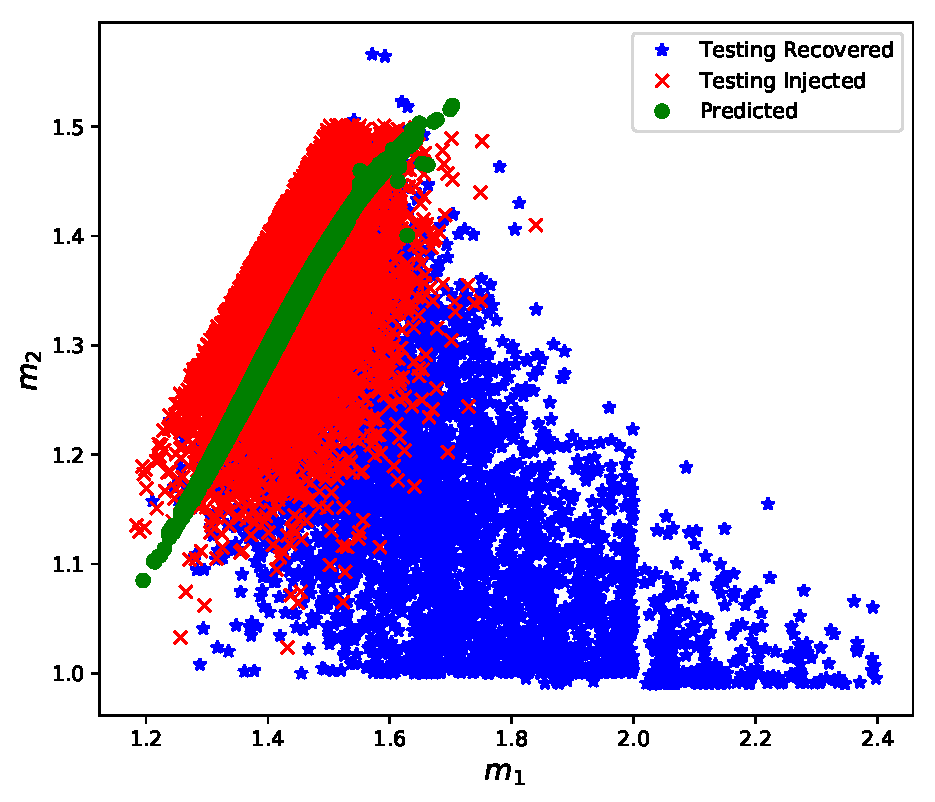
\includegraphics[width=0.45\textwidth]{m1m2_comparison}
  \caption{The $m_1$-$m_2$ parameter space of injections is shown in red, the recovered
  		values from matched-filtering are in blue, and the predicted values from 
		regression are in green.}
\end{figure}

Once the data is read, we prepare it for regression in the following way:
\begin{enumerate}[label=(\roman*)]
	\item Shuffle the data.
	\item Constrain the data to ensure positive values in mass predictions. This requires
	\begin{enumerate}
		\item Mapping the data to be in the range from $(0,1)$. This alone does not
			ensure positive values it is an intermediary step. 
		\item Mapping the data to be in the range from $(-\infty,+\infty)$.
	 \end{enumerate}
	\item Shuffle the data.
	\item Standardize the data so the data has a zero mean and unit variance.
\end{enumerate}

Once the algorithm gives us the predicted data, the reverse process is done, i.e., 
the data is scaled back from standardization, mapped back to $(0,1)$, and exponentiated. 

%==========================================================
\section{Methodology}
%==========================================================

The kernel used for training is the radial basis function (RBF) which is a squared
exponential function given by
\begin{equation}
K(X_1, X_2) = e^{-\frac{||X_1-X_2||^2}{2 \sigma^2}},
\end{equation}
where $X_1$ and $X_2$ are input data points and $\sigma$ is the variance, or lengthscale
parameter. The 
predictions of the \texttt{GstLAL} dataset are independent of kernel choice. However, 
the RBF kernel, apart from its popularity due to its versatility, seems to perform slightly 
better than other kernels and without a loss of speed.

The Adams optimizer is used to find the optimal hyperparameters with a learning rate of 
$0.1$ and $50$ iterations. This combination of learning rate and iterations allows us to 
decrease the marginal log likelihood, or loss, at a quick rate without loss of accuracy. 

Both the \texttt{GstLAL} and O2 datasets are divided as $58\%$ training and $42\%$ 
testing.

%==========================================================
\section{GstLAL Results}
%==========================================================

\begin{figure}[!h]
	\centering
	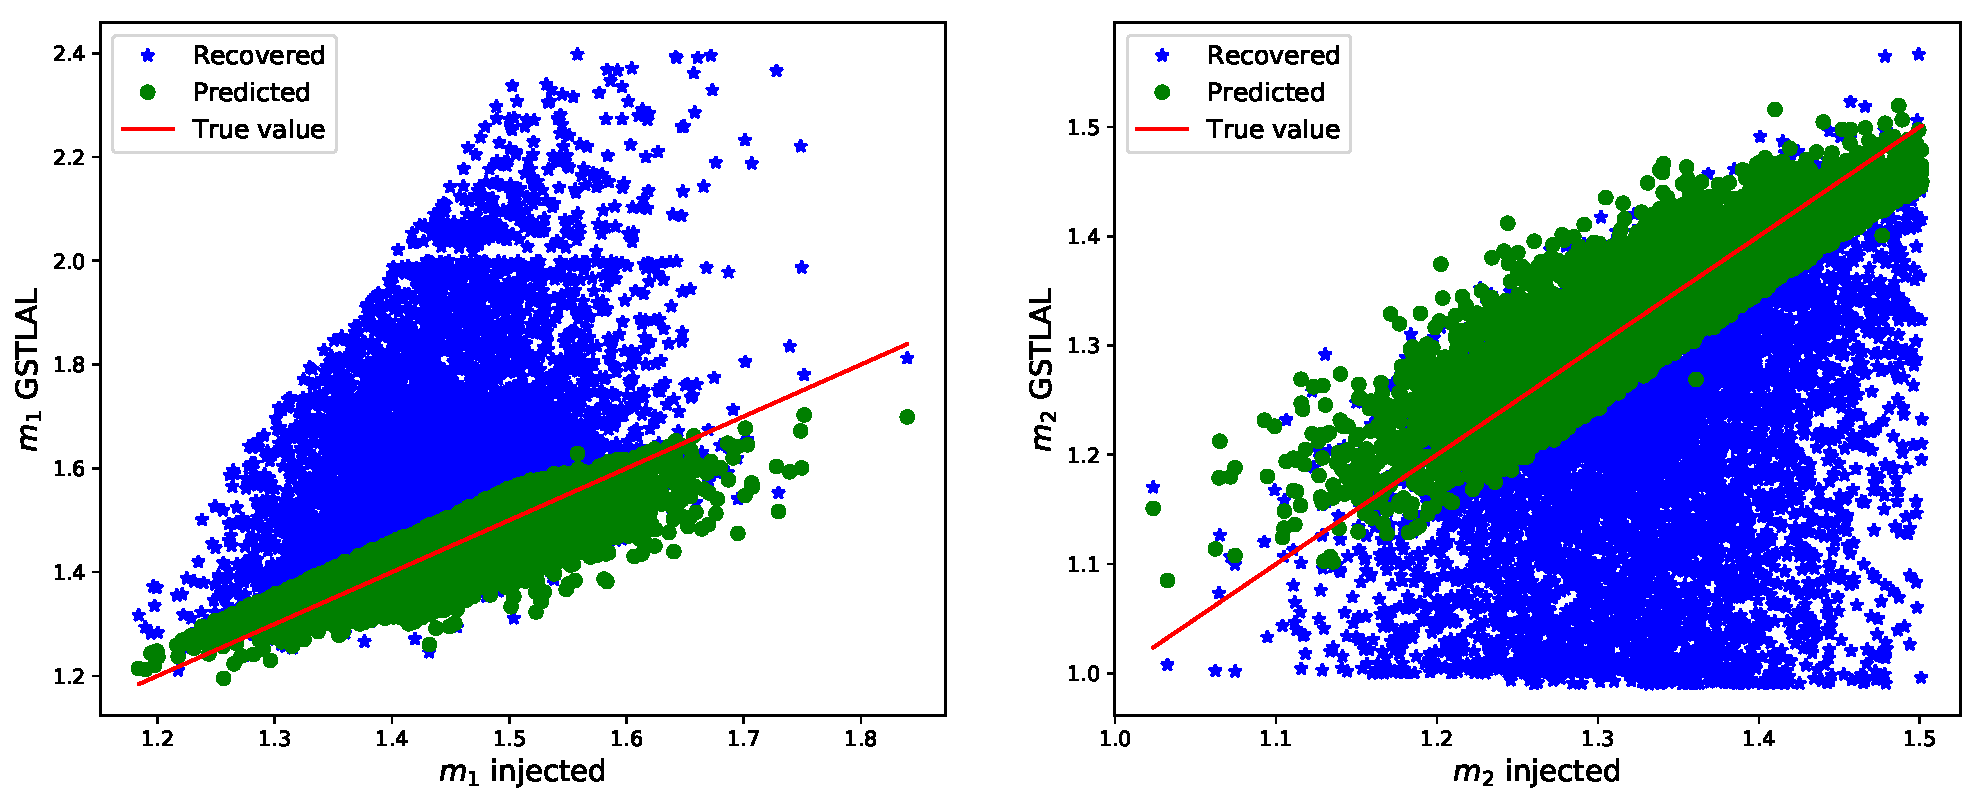
\includegraphics[width=\linewidth]{m1_m2_comparisons}
	\caption{%
	 		The left panel show the injected (red line), recovered (blue stars), and 
			predicted (green circles) values for $m_1$ while the right panel shows the 
			values for $m_2$. Regression is significantly better at producing the true 
			values.}
	\label{fig:regression}
\end{figure}

After running GPR on the datasets, we are able to better predict the masses of the binary 
systems. Fig.~\ref{fig:regression} shows the advantages of using regression. The values of 
the injected masses are depicted by the red line while the recovered masses are shown 
by the blue stars. The predicted masses, shown in green, are much more closely aligned in 
parameters space to the true values. Although the results from GPR are not perfect, the 
comparison between the recovered and predicted values is clear. Moreover, as illustrated in 
Fig.~\ref{fig:fits} the error in the recovery of the primary mass increases as 
the injected $m_1$ increases and the error in the secondary mass decreases as 
the injected $m_2$ value increases. Nevertheless, the error using the predicted values 
stays around zero regardless of the values of the masses injected. 

\begin{figure}[!h]
	\centering
	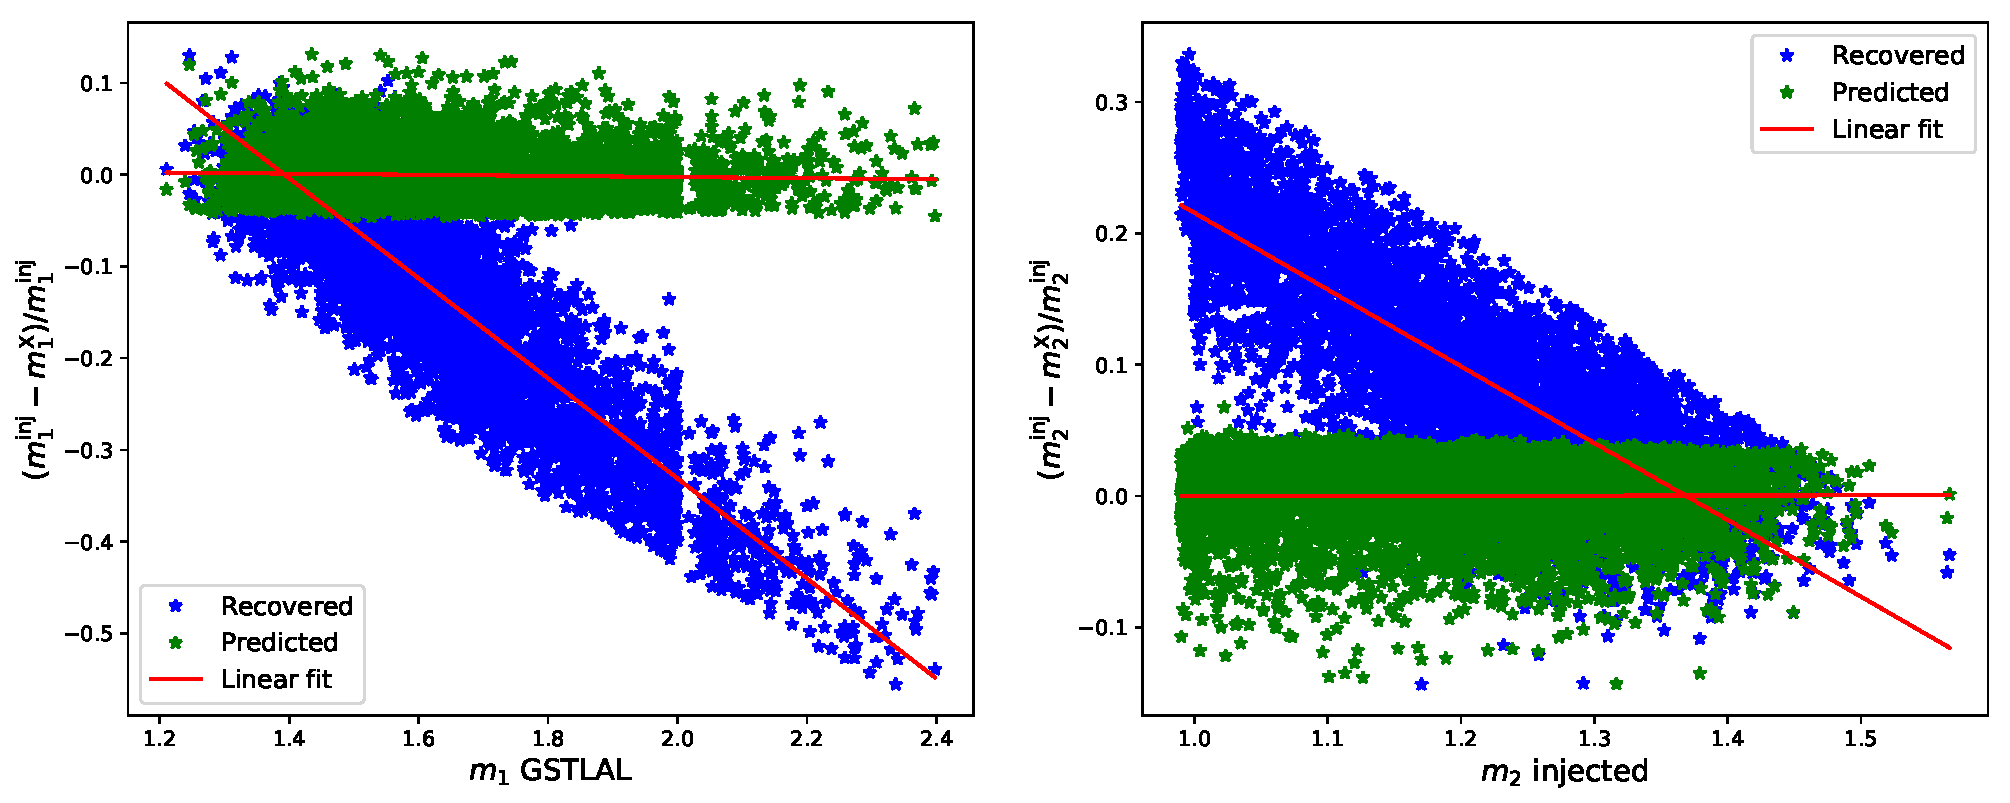
\includegraphics[width=\linewidth]{m1_m2_errors_and_fits}
	\caption{%
	 		The left/right panel show the relative errors in the recovered (blue) and 
			predicted (green) values for $m_1$/$m_2$. The red line is a fit of these values, which 
			shows a relationship between injected $m_1$/$m_2$ values and the recovered and 
			predicted values. GPR has no significant bias that depends on the recovered mass 
			while the \texttt{GstLAL} data does.}
 	\label{fig:fits}
\end{figure}

A different way to visualize Fig.~\ref{fig:fits} is by creating a histogram showing how the 
recovered and predicted values vary from those of the injected values. As seen in 
Fig.~\ref{fig:histogram} the error in the recovered masses is very spread out with errors as high 
as $50\%$. However, using regression allows us to narrow down the errors to no more than 
about $10\%$. Overall, we are able to decrease the mean of the error by as much as three 
orders of magnitudes.

\begin{figure}[!h]
  \centering
  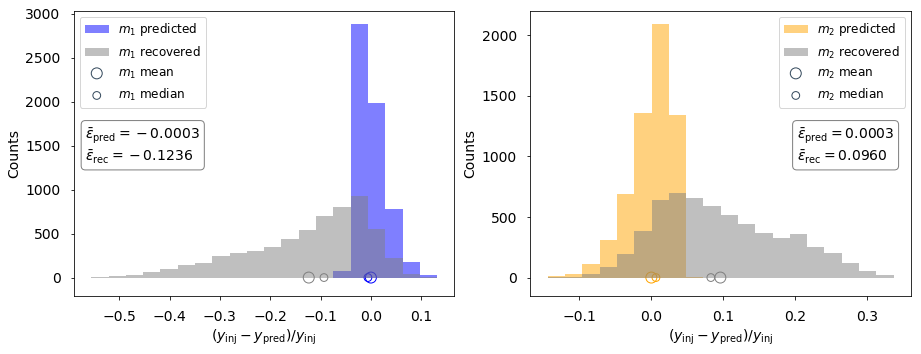
\includegraphics[width=\linewidth]{m1_m2_error_analysis_wboxes}
  \caption{The histogram on the left show the relative error between the injected $m_1$ values and 
  		both the recovered (gray) and predicted (blue) values. Similarly, the right panel shows the 
		relative error between the injected $m_2$ values and both the recovered (gray) and 
		predicted (orange) values. The mean of each dataset is shown by circles on the horizontal 
		axis with the values in boxes. GPR does a great job at decreasing the mean error of the masses. }
  \label{fig:histogram}
\end{figure}

%==========================================================
\subsection{Statistical Analysis}
%==========================================================
%

\begin{figure*}[t]
  \center
  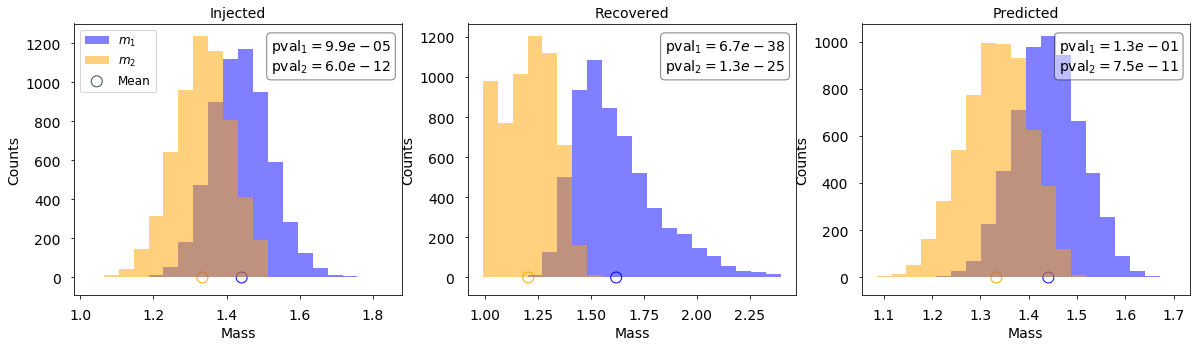
\includegraphics[width=\linewidth]{shapiro_test}
  \caption{The histograms show the mass distributions for the injected (left panel), recovered (middle  
  panel), and predicted (right panel) masses. The p-values corresponding to the Shapiro-Wilk test for 
  normality are printed in the plots. Note that the injected and predicted panels have similar p-values, 
  showing that their distributions are similar in Gaussianity. On the other hand, the recovered p-values 
  are extremely small. This means that they reject the null hypothesis of normality. The distributions 
  are for $N=4,000$ }
  \label{fig:shapiro_test}
\end{figure*}

\textbf{Shapiro-Wilk Test.} To better understand the dataset and the predictions, we perform some 
statistical tests. First, we check for the Gaussianity of the data by performing a Shapiro-Wilk 
test, i.e., by comparing the p-values of the injected, recovered, and predicted values, we are 
able to determine whether the results are normally distributed. Small p-values correspond to 
distributions that are not normal.  As shown in Fig.~\ref{fig:shapiro_test}, the injected 
masses are relatively normal with p-values of $10^{-5}$ and$10^{-12}$ for $m_1$ and 
$m_2$, respectively. Instead the p-values for the recovered masses are on the order of 
$10^{-38}$ and$10^{-25}$ which indicates that the distribution cannot be considered 
``as normal'' as the injected distribution. Furthermore, we use the same test for the predicted 
values and notice that the p-values resemble those of the injected masses. This tells us 
that using regression not only decreases the errors in the masses but also takes us back 
to a distribution similar to the injected one. Therefore, we can say that the predicted values 
agree with the null hypothesis of normality. 

As an extra step, I was interested to see how the p-values change with the amount of data 
included. This is because for more than $5,000$ data points, the p-value test may not be 
accurate. There are a couple of references to add here, but I will come back to that soon. 
Meanwhile, Fig.~\ref{fig:sw_test} show how the p-value changes as one add more data. 
Although the injected and predicted p-values seem to diverge slowly with an increasing 
number of data points, the values are still considered to be similar. Not surprisingly, the 
p-value of the recovered masses reject the null hypothesis that the data is normally 
distributed.
\begin{figure}[h]
  \centering
  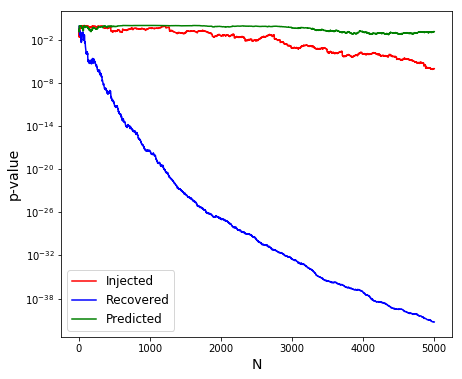
\includegraphics[width=\linewidth]{SW_test}
  \caption{The p-value as a function of number of data points is shown for the injected, 
  		recovered, and predicted data. Note that the p-values between the injected and 
		predicted data sets are always closer together than those of the recovered data.}
  \label{fig:sw_test}
\end{figure}

\textbf{Epps-Singleton Test.} The Epps-Singleton Test allows us to check if two 
sets of data have the same underlying probability distribution. A p-value of $1$ means 
that two set of data have the same probability distribution while a p-value of $0$ tells us 
that the two datasets are completely different in their distributions. When comparing the 
injected and recovered values, the p-value is $2.5*10^{-22}$. On the other hand, comparing 
the injected and predicted values gives us a p-value of $0.32$. 

\textbf{Kolmogorov-Smirnov Test.} This last test compares the underlying continuous 
distributions of two independent samples. What we find that that the p-value for the 
injected and recovered distributions is $0$, i.e., the distribution of the injected values are 
not equal to the distribution of the recovered values. Instead for the predicted values, we get 
a p-value of $0.002$ which tells us that although the continuous distributions are not the 
same, they are not completely different since there is some overlap. Fig.~\ref{fig:ks_test} 
shows the distribution of data as a function of mass. This visual shows us clearly that the 
recovered values for $m_1$ tend to overestimate the mass and the recovered $m_2$ 
values mostly underestimate the mass. This is corroborated by calculating the p-values. 
For example, the p-value between the injected and recovered $m_1$ is $1$ when the 
null hypothesis is that the underlying distribution of the injected parameters is less than 
the underlying distribution of the recovered parameters. In other words, the recovered 
masses overestimate the values. The converse gives us a p-value of $0$. If instead we turn 
our attention to the right panel of Fig.~\ref{fig:ks_test}, we can test for the distribution of 
the $m_2$ values. The p-value between the injected and recovered $m_2$ is $1$ when the 
null hypothesis is that the underlying distribution of the injected parameters is greater than 
the underlying distribution of the recovered parameters. When comparing the predicted data, 
however, the p-values are small but not so small that any null hypothesis can be rejected. 
``Any'' meaning that the continuous distribution of the predicted values is similar to the 
injected values.
\begin{figure*}[t]
  \centering
  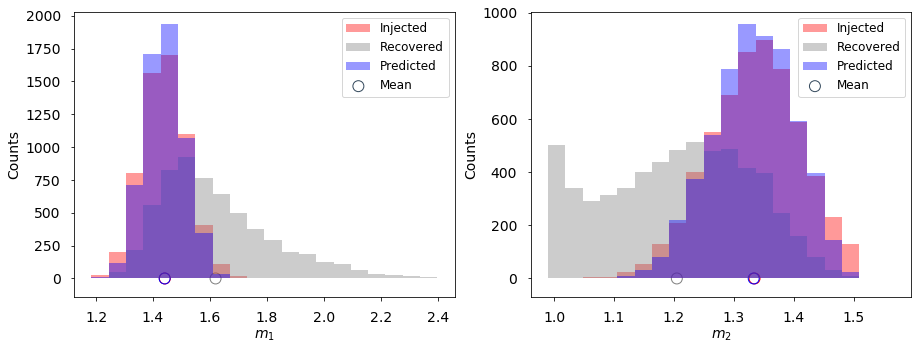
\includegraphics[width=\linewidth]{KS_test}
  \caption{The panels show the mass distributions for the injected, recovered, and predicted 
  		datasets. This hints at the biases in the recovered data.}
  \label{fig:ks_test}
\end{figure*}

%==========================================================
\section{O2 Data Results}
%==========================================================
The same analysis will be done with the O2 data, which is currently running. 
Meanwhile, $1/7$ of the data has been analysed and results do not look too good. 
However, better results are expected since these partial results represent a mass 
range that is $100$ times larger than the previous test dataset. Stay tuned!

%==========================================================
%\section{Conclusions}
%==========================================================


\end{document}